% V6 mechanism manuscript: complete two-localizer analyses are required below.
% The previous v5 sources, PDFs and experimental receipts remain unchanged.
\documentclass[10pt,twocolumn,letterpaper]{article}
\usepackage[review]{cvpr}
% Minimal empirical-study preamble; no historical model macros or number registry.
\usepackage[T1]{fontenc}
\usepackage{times}
\usepackage{amsmath,amssymb}
\usepackage{booktabs}
\usepackage{graphicx}
\usepackage{multirow}
\usepackage{xcolor}
\usepackage{microtype}
\usepackage{enumitem}
\usepackage{placeins}

\definecolor{cvprblue}{rgb}{0.21,0.49,0.74}
\usepackage[pagebackref,breaklinks,colorlinks,allcolors=cvprblue]{hyperref}
\def\paperID{*****}\def\confName{CVPR}\def\confYear{2027}
% Generated only after all 18 new heads and all three analysis surfaces finish.
% Complete analyses validated; this is not a submission-readiness certificate.
\def\ReadoutV6AssetsComplete{1}

\title{Confidence for Which Prediction?\\
Supervision Targets and Query Readout in Visual Grounding}
\author{Anonymous submission}
\begin{document}\maketitle
\begin{abstract}
Grounding confidence must reject absent referents and detect wrong boxes.
We cross existence/correct-emission supervision with global-max/selected-query
readouts on two frozen grounders, matching heads and training while keeping
every output box fixed.
For MM-GDINO-T, emission-minus-existence supervision under global readout changes correct-versus-wrong-box AUROC by +11.654 points but mixed AUGRC by +0.149 [+0.058, +0.235].
For MDETR-R101, emission-minus-existence supervision under global readout changes correct-versus-wrong-box AUROC by +13.889 points but mixed AUGRC by -0.866 [-0.988, -0.745].

Existence AUROC declines in both systems, although complete-risk changes
have opposite signs. Selected-query scoring does not consistently favor
emission supervision, and transfer can reverse its gains. Three-state
decomposition explains the relevant comparisons; fixed combinations show
that practical gains depend on the population and reference score.
\end{abstract}

\begin{figure*}[t]
\centering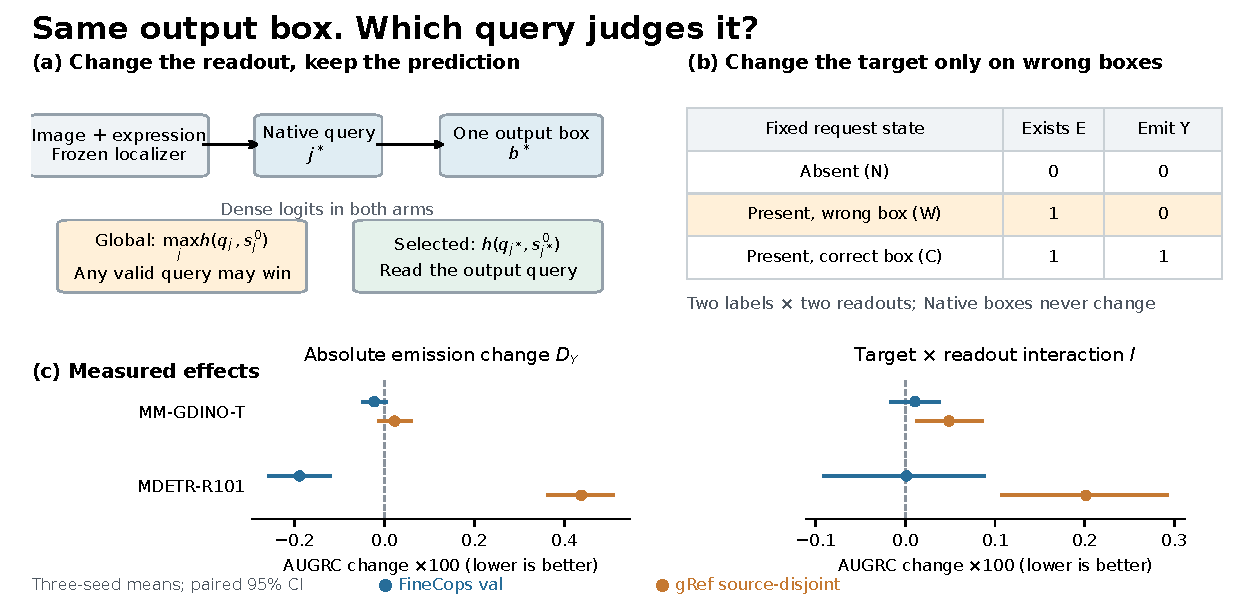
\includegraphics[width=\textwidth]{generated/readout_v6/figure1_readout.pdf}
\caption{\textbf{Same output box. Which query judges it?}
(a) Native always selects the output. The learned confidence either reads
the largest logit across queries ($G$) or the Native-selected query ($S$).
(b) Existence ($E$) and correct-emission ($Y$) supervision differ only on
present-but-wrong requests. (c) For mixed AUGRC $R$,
$D_Y=R_{S,Y}-R_{G,Y}$ and $D_E=R_{S,E}-R_{G,E}$ are absolute readout changes;
$I=D_Y-D_E$ is their target interaction. Neither $D_Y$ nor $I$ substitutes
for the other. Results are three-seed means with paired image-cluster
95\% intervals. A change of readout also changes query competition and
training-gradient routing; spatial correspondence is a hypothesis, not a
consequence of the diagram.}
\label{fig:readout_question}
\end{figure*}

\section{Introduction}
A visual grounding system must locate the object described by an expression
and decide when to return no box. Two failures matter: a plausible expression
may have no referent, and an existing referent may be localized incorrectly.
Distinguishing valid from invalid requests is therefore not the same task
as recognizing reliable outputs. This difference is consequential in
generalized grounding, where a user can refer to an absent object and
every accepted wrong localization remains a failure
\cite{he2023grec,liu2023gres,liu2024finecops}.

A natural response is to supervise exactly the event desired at deployment:
the target exists \emph{and} the emitted box is correct. With the true
conditional success probability, ranking by this event would optimally
prioritize successes at a fixed coverage under equal failure costs.
Finite learned heads, however, need not estimate that probability.
Their representation and readout determine which evidence is available
and where supervision acts; training coverage also limits which request
patterns receive direct supervision and which require generalization.
The substantive question is therefore not
whether correct-output supervision is intrinsically contradictory, but
\emph{why it can be insufficient in a concrete grounding confidence design}.

Query-based grounding makes one explanation directly testable. The system's
Native score selects a particular box, while a learned global-max confidence
can be supplied by another query. Any query may provide evidence that a
referent exists; confidence in \emph{the chosen prediction} may instead
benefit from reading its query. Yet replacing global max with a selected
query changes more than geometric correspondence: it removes max competition
and redirects the training gradient. Treating an improved selected-query
endpoint as proof of spatial alignment would skip these distinctions.

We cross supervision target with query readout while fixing the localizer,
output boxes, confidence-head architecture, initialization, samples and
optimization. The resulting $2\times2$ identifies target effects within
each readout and readout effects within each target. We report both the
absolute change in emission risk and the difference of target effects;
a negative interaction alone can arise because the existence head gets
worse. A second localizer and frozen transfer answer different scope
questions, so neither is used as a substitute for the other.

The findings do not support a general selected-query repair or an
inevitable supervision tradeoff. On MM-GDINO's FineCops validation surface, the emission head's risk
disadvantage survives reading exactly the emitted query. On MDETR,
emission supervision lowers complete-output risk even while existence
AUROC falls. Reading the selected query improves both MDETR heads on
FineCops, but its frozen transfer worsens emission risk on gRefCOCO.
The important distinction is therefore which successful-output
comparisons change, not whether a confidence score has gained or lost
existence AUROC alone.

The explanation then follows the failures that complete output risk
actually counts. We separately compare correct boxes against wrong boxes,
correct boxes against no-target requests, and wrong boxes against no-targets.
An exact generalized-risk identity makes the first two comparisons explicit
and identifies when a request-prior change can reverse a score preference.
Same-image, parent-pair and difficulty-conditioned analyses test whether
these effects remain within comparable grounding requests. Finally, two
fixed combinations of Native and existence scores ask whether an observed
tradeoff between individual scores has to become a practical design choice.

Our contribution is a controlled account of \emph{supervision--readout
interaction and its boundaries}: (i) a matched target-by-readout
intervention on two frozen grounding systems, with frozen-head transfer;
and (ii) a three-state explanation connecting the measured changes to
complete output risk, conditional comparisons and fixed combinations.
A record-only evaluator accompanies the results to support reuse with
other fixed localizers and confidence scores.

\section{Related Work}
\paragraph{Grounding beyond guaranteed referents.}
Grounding DINO \cite{liu2025groundingdino} and MDETR \cite{kamath2021mdetr}
provide language-conditioned query representations but differ in
architecture, pretraining, adaptation and candidate count.
GREC and gRefCOCO permit no-target and multiple-target requests
\cite{he2023grec,liu2023gres}; FineCops adds compositional positives and
negative expressions/images \cite{liu2024finecops}. We study single/no-target
requests and fix one emitted box per localizer. Unlike a positive-only
grounding comparison, the resulting failure event includes both
mislocalization and an unnecessary output.

\paragraph{Prediction quality and selective risk.}
Learning localization-aware detection scores is established
\cite{li2020gfl}, as is learning a reject option with a predictor
\cite{geifman2019selectivenet}. Calibration concerns score values and
operating points, including their stability under shift
\cite{guo2017calibration,ovadia2019trust}. Our primary question concerns
ranking fixed predictions by complete-output reliability; we neither
improve their boxes nor fit an operational threshold on the evaluation
populations.

\paragraph{Joint failure detection.}
Misclassification and out-of-distribution detection are distinct, and
evaluating an incomplete failure population can mislead
\cite{jaeger2023failure}. OpenMix \cite{zhu2023openmix} and SCOD
\cite{narasimhan2024scod} address joint objectives; SIRC explicitly
studies combining confidence information and sensitivity to failure
mixtures and costs \cite{xia2024sirc}. AUGRC addresses limitations of
conventional selective-risk integration \cite{traub2024augrc}.
We do not claim that three failure states, mixed-population preference
changes or combining complementary scores are new general principles.
Our independent question is how a matched \emph{supervision intervention}
interacts with a grounding system's \emph{query readout}. The spatial
winner and same-image/edited-expression analyses turn grounding-specific
structure into testable evidence, rather than relying on task context
alone. Our SIRC-style combination is a fixed, training-statistics-based
control, not a complete reimplementation of every SIRC estimator.

\section{Controlled Study}
\subsection{Fixed output, crossed target and readout}
For an image--expression request, localizer $L$ produces frozen query
features $q_j$, scores $s_j^0$ and boxes $b_j$. Its Native selector yields
$j^*$ and $b^*=b_{j^*}$. The selector includes the localizer's own
tie convention; confidence never enters it.

The three states are no target ($N$), present but Native-wrong ($W$),
and present with Native IoU at least $0.5$ ($C$).
Existence supervision uses $E=1$ on $C,W$ and zero on $N$.
Emission supervision uses $Y=1$ only on $C$. Both see the same requests;
only the label on $W$ changes. No-target requests receive no fabricated GT.

Each head computes dense logits
$z_j=h([\operatorname{detach}(q_j);
\operatorname{detach}(s_j^0)])$. Its request score is either
\begin{equation}
 c_G=\max_{j\in\mathcal V}z_j,\qquad c_S=z_{j^*}.
\end{equation}
The same readout is used in training and matched evaluation. We also save
both readouts of each trained head for a frozen-weight diagnostic.
This separates inference re-reading from retraining along an explicit
path, without claiming a unique additive decomposition of spatial and
optimization effects.

\subsection{Localizers and matched head training}
The first localizer is the fixed five-epoch positive-source FineCops
MM-GDINO-T artifact, with 900 256-d queries.
The second is the official RefCOCO MDETR-R101 EMA checkpoint, with
100 256-d queries. Each supplies its own Native scores, selector and
correctness labels. The models are not a pure architecture intervention:
their training lineage, candidate count and Native accuracy differ.
They test the applicability of the \emph{within-localizer} control.

All heads use LayerNorm(257), linear layers
$257\rightarrow128\rightarrow128\rightarrow1$, GELU hidden activations,
and a zero-initialized final layer: 50,179 parameters in eight tensors.
Initialization is copied across arms within each seed 17/42/73.
Both readouts compute the full dense head before max/gather.
Five epochs give 12,575 updates on the same 80,451 FineCops training
pairs, with batch 32 pairs, AdamW LR $10^{-4}$, WD=0 and clip 0.1.
Each source contributes half the mean BCE, with the same $10^{-3}$
source-averaged squared-logit penalty. No emit-specific resampling or
class weighting is added. FP32 deterministic head computation uses
FP16 cached features and FP32 Native scores/boxes.

\paragraph{Supervision coverage.}
The 80,451 training pairs draw their positives from 43,979 unique L1
parents; no L2 or L3 positive enters the confidence-head loss.
The full 83,341-positive cache is used for SIRC score normalization,
not additional head-loss coverage, while the MM-GDINO trunk was
adapted on the full positive-source population.
Validation covers L1--L3, but every one of its 9,029 negative-text
requests has an L1 positive parent. All target/readout arms retain
this same coverage; the matrix does not match training and evaluation
complexity support.

The original six MM-GDINO global heads are reused unchanged; six
selected heads and twelve MDETR heads are new. All 18 new heads reach
the fixed endpoint before transfer. Trunks and unused rank parameters
remain frozen, and all evaluated confidence routes preserve the Native
prediction exactly.

\subsection{Populations and inference}
FineCops validation supplies 9,426 positives and 9,029 text negatives.
Frozen transfer uses gRefCOCO TestA/B single/no-target requests:
11,563 positives and 9,121 no-targets on 1,500 images.
All 14,579 multi-target expressions are excluded.
The source-disjoint sensitivity removes FineCops train/validation
source images using VG--COCO identities or exact image bytes, leaving
1,277 images, 9,848 positives and 7,716 no-targets.
This is source-disjointness from the current FineCops populations,
not global pretraining image-disjointness.
In particular, MDETR's RefCOCO adaptation and gRefCOCO share the
COCO source domain; this exclusion does not audit away that lineage.

Full expressions enter each localizer, without support patches,
category replacement, NMS changes or a confidence-selected box.
One cached detector traversal per localizer serves every head.
Native and the six reused MM-GDINO heads must reproduce their
previous records bitwise, including original head-batch grouping.
These are post-hoc-motivated, prospectively locked mechanism experiments
on previously investigated benchmarks. FineCops Test is not reopened;
no checkpoint, Gap or deployment threshold is selected.

\subsection{Primary effects and uncertainty}
Our complete-output metric is AUGRC
\cite{traub2024augrc}, integrating
$\Pr(Y=0,c\geq t)$ over coverage. It penalizes both accepted $W$
and accepted $N$. Conventional mixed/positive AURC, existence AUROC,
three-state AUROCs, diagnostic FPR95 and fixed-coverage failure
composition are retained.

For observed-mixture AUGRC $R$, define
\begin{align}
D_Y&=R_{S,Y}-R_{G,Y},\quad D_E=R_{S,E}-R_{G,E},\nonumber\\
I&=(R_{S,Y}-R_{S,E})-(R_{G,Y}-R_{G,E})\nonumber\\
 &=D_Y-D_E.
\end{align}
A negative $D_Y$ is an absolute emission improvement; a negative $I$
indicates that selected readout benefits emission \emph{relative to}
existence. We report both magnitudes and paired intervals, rather than
substituting a sign test on one for the other.

All contrasts use 5,000 paired image-cluster draws with PCG64 seed
20260911. One image draw is shared across both localizers, every score
and all three seeds; metrics are recomputed per seed before equal
averaging. gRef draws are stratified by TestA/B. Intervals are
exploratory 95\% percentile intervals conditional on frozen checkpoints;
seed sample SD is separate. FPR95 recalculates each score's positive
q05 inside every draw, not an operational threshold.

\begin{table*}[t]
\centering\small
\setlength{\tabcolsep}{3pt}
\renewcommand{\arraystretch}{1.15}
\caption{Target by readout with unchanged Native boxes. Mixed AUGRC $\times100$ (lower is better). The four cells show seed mean (sample SD); effects show mean [paired 95\% CI]. $D_Y=R_{S,Y}-R_{G,Y}$, $D_E=R_{S,E}-R_{G,E}$, and $I=D_Y-D_E$. The gRef surfaces overlap and are not independent replications.}\label{tab:readout_matrix}
\begin{tabular}{@{}llccccccc@{}}\toprule
Localizer & Population & $G/E$ & $G/Y$ & $S/E$ & $S/Y$ & $D_Y$ & $D_E$ & $I$\\\midrule
MM-GDINO-T & FineCops val & \shortstack{26.23\\{\scriptsize (0.07)}} & \shortstack{26.38\\{\scriptsize (0.04)}} & \shortstack{26.20\\{\scriptsize (0.07)}} & \shortstack{26.36\\{\scriptsize (0.04)}} & \shortstack{-0.023\\{\scriptsize [-0.048, +0.003]}} & \shortstack{-0.034\\{\scriptsize [-0.068, +0.000]}} & \shortstack{+0.011\\{\scriptsize [-0.016, +0.038]}}\\
MM-GDINO-T & gRef source-disjoint & \shortstack{28.68\\{\scriptsize (0.08)}} & \shortstack{28.61\\{\scriptsize (0.04)}} & \shortstack{28.65\\{\scriptsize (0.11)}} & \shortstack{28.63\\{\scriptsize (0.05)}} & \shortstack{+0.022\\{\scriptsize [-0.013, +0.057]}} & \shortstack{-0.027\\{\scriptsize [-0.060, +0.007]}} & \shortstack{+0.049\\{\scriptsize [+0.013, +0.085]}}\\
MM-GDINO-T & gRef Full & \shortstack{28.79\\{\scriptsize (0.08)}} & \shortstack{28.75\\{\scriptsize (0.05)}} & \shortstack{28.76\\{\scriptsize (0.11)}} & \shortstack{28.76\\{\scriptsize (0.05)}} & \shortstack{+0.011\\{\scriptsize [-0.021, +0.045]}} & \shortstack{-0.025\\{\scriptsize [-0.055, +0.006]}} & \shortstack{+0.037\\{\scriptsize [+0.003, +0.069]}}\\
\addlinespace[3pt]
MDETR-R101 & FineCops val & \shortstack{29.71\\{\scriptsize (0.27)}} & \shortstack{28.84\\{\scriptsize (0.13)}} & \shortstack{29.52\\{\scriptsize (0.28)}} & \shortstack{28.65\\{\scriptsize (0.02)}} & \shortstack{-0.189\\{\scriptsize [-0.257, -0.122]}} & \shortstack{-0.191\\{\scriptsize [-0.285, -0.094]}} & \shortstack{+0.001\\{\scriptsize [-0.091, +0.088]}}\\
MDETR-R101 & gRef source-disjoint & \shortstack{20.11\\{\scriptsize (0.54)}} & \shortstack{19.92\\{\scriptsize (0.38)}} & \shortstack{20.34\\{\scriptsize (0.15)}} & \shortstack{20.35\\{\scriptsize (0.06)}} & \shortstack{+0.437\\{\scriptsize [+0.363, +0.507]}} & \shortstack{+0.236\\{\scriptsize [+0.137, +0.332]}} & \shortstack{+0.201\\{\scriptsize [+0.108, +0.292]}}\\
MDETR-R101 & gRef Full & \shortstack{20.25\\{\scriptsize (0.53)}} & \shortstack{20.09\\{\scriptsize (0.39)}} & \shortstack{20.52\\{\scriptsize (0.14)}} & \shortstack{20.53\\{\scriptsize (0.06)}} & \shortstack{+0.440\\{\scriptsize [+0.373, +0.506]}} & \shortstack{+0.268\\{\scriptsize [+0.176, +0.356]}} & \shortstack{+0.172\\{\scriptsize [+0.085, +0.259]}}\\
\addlinespace[3pt]
\bottomrule\end{tabular}
\end{table*}


\section{Does Readout Change the Supervision Effect?}
\paragraph{MM-GDINO-T on FineCops.} Native P@1 is 77.36\%, unchanged across every confidence route. The absolute emission change is $D_Y=-0.023 [-0.048, +0.003]$ points; the existence change is $D_E=-0.034 [-0.068, +0.000]$, and $I=+0.011 [-0.016, +0.038]$. Emission risk decreases in the point estimate without a negative target-specific interaction; a general readout effect is distinct from an emission-specific advantage.

\paragraph{MDETR-R101 on FineCops.} Native P@1 is 65.56\%, unchanged across every confidence route. The absolute emission change is $D_Y=-0.189 [-0.257, -0.122]$ points; the existence change is $D_E=-0.191 [-0.285, -0.094]$, and $I=+0.001 [-0.091, +0.088]$. Emission risk decreases in the point estimate without a negative target-specific interaction; a general readout effect is distinct from an emission-specific advantage.


On MM-GDINO FineCops validation, the emission-minus-existence risk disadvantage remains
under both matched readouts. It therefore does not require a confidence
score supplied by a query different from the emitted one. The MDETR
result illustrates the other distinction: both targets improve by
similar amounts under Selected, without a resolved emission-specific
interaction. This is evidence about the readout intervention, not an
identified spatial-alignment contribution or an equivalence result.

The four-cell comparison therefore distinguishes absolute readout gains
from an advantage specific to emission supervision.

\section{Which State Comparisons Explain Output Risk?}
\begin{table*}[t]
\centering\small
\setlength{\tabcolsep}{3pt}
\renewcommand{\arraystretch}{1.15}
\caption{The same existence-AUROC change need not imply the same output-risk change. Emission-minus-existence effects $\times100$ [paired 95\% CI]; positive denotes larger AUROC, negative denotes lower AUGRC. $C/W$ tests localized correctness, $C/N$ tests successful outputs against absent targets, and $W/N$ compares two failures. The first two determine fixed-population AUGRC, whereas existence AUROC also includes the third. Readout contrasts and gRef Full are retained in Table~\ref{tab:readout_matrix} and the complete analysis.}\label{tab:readout_states}
\begin{tabular}{@{}lllccccc@{}}\toprule
Localizer & Population & Readout & $C/W$ & $C/N$ & $W/N$ & Existence & AUGRC\\\midrule
MM-GDINO-T & FineCops val & $G$ & \shortstack{+11.654\\{\scriptsize [+10.721, +12.641]}} & \shortstack{-3.523\\{\scriptsize [-3.884, -3.166]}} & \shortstack{-17.795\\{\scriptsize [-18.821, -16.781]}} & \shortstack{-6.754\\{\scriptsize [-7.211, -6.308]}} & \shortstack{+0.149\\{\scriptsize [+0.058, +0.235]}}\\
MM-GDINO-T & FineCops val & $S$ & \shortstack{+10.724\\{\scriptsize [+9.850, +11.606]}} & \shortstack{-3.359\\{\scriptsize [-3.700, -3.019]}} & \shortstack{-16.823\\{\scriptsize [-17.738, -15.898]}} & \shortstack{-6.408\\{\scriptsize [-6.827, -5.984]}} & \shortstack{+0.159\\{\scriptsize [+0.077, +0.241]}}\\
MM-GDINO-T & gRef source-disjoint & $G$ & \shortstack{+6.533\\{\scriptsize [+5.605, +7.467]}} & \shortstack{-3.184\\{\scriptsize [-3.635, -2.751]}} & \shortstack{-7.204\\{\scriptsize [-7.895, -6.501]}} & \shortstack{-4.951\\{\scriptsize [-5.398, -4.511]}} & \shortstack{-0.066\\{\scriptsize [-0.178, +0.043]}}\\
MM-GDINO-T & gRef source-disjoint & $S$ & \shortstack{+6.056\\{\scriptsize [+5.198, +6.931]}} & \shortstack{-3.270\\{\scriptsize [-3.706, -2.853]}} & \shortstack{-7.774\\{\scriptsize [-8.476, -7.074]}} & \shortstack{-5.250\\{\scriptsize [-5.706, -4.806]}} & \shortstack{-0.018\\{\scriptsize [-0.127, +0.090]}}\\
MDETR-R101 & FineCops val & $G$ & \shortstack{+13.889\\{\scriptsize [+13.044, +14.743]}} & \shortstack{+0.290\\{\scriptsize [-0.265, +0.857]}} & \shortstack{-14.257\\{\scriptsize [-15.124, -13.406]}} & \shortstack{-4.719\\{\scriptsize [-5.271, -4.165]}} & \shortstack{-0.866\\{\scriptsize [-0.988, -0.745]}}\\
MDETR-R101 & FineCops val & $S$ & \shortstack{+14.622\\{\scriptsize [+13.664, +15.565]}} & \shortstack{+0.017\\{\scriptsize [-0.577, +0.618]}} & \shortstack{-15.673\\{\scriptsize [-16.619, -14.698]}} & \shortstack{-5.386\\{\scriptsize [-5.977, -4.774]}} & \shortstack{-0.864\\{\scriptsize [-0.993, -0.737]}}\\
MDETR-R101 & gRef source-disjoint & $G$ & \shortstack{+6.204\\{\scriptsize [+5.153, +7.325]}} & \shortstack{-0.493\\{\scriptsize [-0.917, -0.082]}} & \shortstack{-7.990\\{\scriptsize [-9.622, -6.478]}} & \shortstack{-1.844\\{\scriptsize [-2.322, -1.395]}} & \shortstack{-0.189\\{\scriptsize [-0.291, -0.083]}}\\
MDETR-R101 & gRef source-disjoint & $S$ & \shortstack{+4.992\\{\scriptsize [+3.774, +6.338]}} & \shortstack{-1.211\\{\scriptsize [-1.707, -0.698]}} & \shortstack{-7.151\\{\scriptsize [-8.950, -5.463]}} & \shortstack{-2.281\\{\scriptsize [-2.833, -1.738]}} & \shortstack{+0.013\\{\scriptsize [-0.119, +0.138]}}\\
\bottomrule\end{tabular}
\end{table*}

Let $U_{CW},U_{CN},U_{WN}$ be pairwise AUROCs with half credit for
equal scores, and let $a=\Pr(C\mid E=1)$. Then
\begin{equation}
\operatorname{AUC}_E=aU_{CN}+(1-a)U_{WN}.
\end{equation}
Existence AUROC therefore includes a comparison between two failures.
Its decrease does not by itself identify which discrimination needed
for successful outputs was lost.

For no-target prior $\pi$, the masses of $C,W,N$ are
$(1-\pi)a,(1-\pi)(1-a),\pi$. With Native predictions held fixed, the
difference between any two score rules obeys
\begin{align}
\Delta\operatorname{AUGRC}
=-(1-\pi)a\big[&(1-\pi)(1-a)\Delta U_{CW}\nonumber\\
&+\pi\Delta U_{CN}\big].
\label{eq:state_risk}
\end{align}
Thus $C/W$ and $C/N$, not $W/N$, determine the change in complete
risk. The identity exposes the crossing condition when these two
effects oppose. An interior crossover is reported only when it exists;
bootstrap draws without one are retained, not forced into an interval.
This is an AUGRC identity, not a formula for AURC or a newly claimed
general principle of prior sensitivity.

\paragraph{MM-GDINO-T on FineCops.} Under global readout, emission-minus-existence changes $U_{CW}$ by +11.654 [+10.721, +12.641] AUROC points and $U_{CN}$ by -3.523 [-3.884, -3.166]. Existence AUROC changes by -6.754 [-7.211, -6.308], whereas complete-output AUGRC changes by +0.149 [+0.058, +0.235]. At the point estimate, the $C/W$ and $C/N$ risk contributions are -0.532 and +0.681 AUGRC points, respectively. Their sum, not the $W/N$ comparison, reconstructs the risk change.

\paragraph{MDETR-R101 on FineCops.} Under global readout, emission-minus-existence changes $U_{CW}$ by +13.889 [+13.044, +14.743] AUROC points and $U_{CN}$ by +0.290 [-0.265, +0.857]. Existence AUROC changes by -4.719 [-5.271, -4.165], whereas complete-output AUGRC changes by -0.866 [-0.988, -0.745]. At the point estimate, the $C/W$ and $C/N$ risk contributions are -0.818 and -0.047 AUGRC points, respectively. Their sum, not the $W/N$ comparison, reconstructs the risk change.

\paragraph{What changes among accepted requests?} At approximately 50\% coverage on MM-GDINO FineCops, global emission supervision changes the accepted wrong-box fraction from 8.44\% to 3.55\%, while the accepted no-target fraction changes from 41.46\% to 46.81\%. Both denominators are accepted requests, not their respective failure classes. The fixed-coverage supplement gives achieved coverage and paired intervals.


These models share an existence-AUROC decline, but not the same
complete-output consequence. For MM-GDINO, the resolved $C/N$ loss
outweighs its $C/W$ benefit at the observed mixture. For MDETR, the
$C/N$ change is small and unresolved, while the $C/W$ benefit lowers
complete risk. Its large $W/N$ decrease reduces existence AUROC without
directly penalizing the binary successful-output ranking. A falling
existence AUROC is therefore insufficient evidence of a reliability
tradeoff, even within this matched supervision experiment.

\paragraph{Testing finer explanations.}
Winner indices alone do not establish a spatial mismatch: different
queries can predict nearly identical boxes. We therefore record
winner--Native box IoU and both winners' GT IoU, including the case
where Native is wrong but the confidence winner is spatially correct.
Here every diagnostic winner is the dense-logit global argmax.
It supplies matched confidence for $G$, but is a counterfactual
diagnostic for $S$: deployed $S$ always reads the Native query and
has zero readout-index disagreement.
Frozen-weight alternate readouts complement, rather than replace,
the matched training comparison.
On MM-GDINO FineCops validation, the global-emission winner already
matches Native's query on approximately 95\% of correct positives and
82\% of wrong positives. Among Native-wrong positives, about 9\% have
a spatially correct confidence winner. Such cases establish a real
distinction between evidence for a referent and evidence for the emitted
box; they do not identify its share of the endpoint effect.

We also condition $C/W$, $C/N$ and $W/N$ comparisons on shared images
and original positive-expression difficulty. FineCops provides actual
edited-negative/parent-positive pairs; gRef provides same-image
comparisons, not edited-expression counterfactuals. Same-image
conditional effects use the \emph{same participating requests} as their
unconditional reference. Difficulty conditioning instead restricts
the available within-level state pairs; it is not an exactly matched
target distribution. An interval crossing zero means insufficient
resolution, not evidence that an image/difficulty explanation accounts
for the effect. The supplement reports attenuation, uncertainty,
sample counts and all winner diagnostics without assigning a unique
spatial contribution.
% Source: finecops_val.json / mmgdino_positive / global_emit_minus_exists;
% same_image_cn{,_comparable_unconditional}, difficulty_cn_level1,
% difficulty_cn_cross_level_contribution. AUROC differences multiplied by 100.
For MM-GDINO's global target contrast, the $C/N$ loss remains within
images: $-1.163$ [$-1.557,-0.760$] AUROC points, compared with
$-1.700$ [$-2.002,-1.400$] unconditionally on the same participating
requests. It is therefore not confined to cross-image comparisons.
Within L1, however, the $C/N$ change is $+0.224$
[$+0.024,+0.431$]; the cross-level contribution is
$-3.692$ [$-4.019,-3.384$]. This localizes the difficulty structure
of the aggregate change without making it a causal explanation.
Because all negative parents are L1, the same-difficulty $C/N$ and
$W/N$ comparisons exist only at L1. Their cross-level counterparts
compare L2/L3 positives, which receive no direct head-loss supervision,
against L1-parent negatives. This identifies a coverage boundary and
the compared populations, not a causal attribution of the measured loss.

\section{Do the Effects Extend Beyond One Setting?}
\paragraph{MM-GDINO-T, gRef source-disjoint.} Native P@1 is 56.04\%. The frozen-head emission readout effect is +0.022 [-0.013, +0.057] AUGRC points, and its target interaction is +0.049 [+0.013, +0.085]. This population does not show an absolute emission-risk improvement in the point estimate. The magnitudes and paired intervals, rather than an interaction sign alone, determine its scope.

\paragraph{MDETR-R101, gRef source-disjoint.} Native P@1 is 81.98\%. The frozen-head emission readout effect is +0.437 [+0.363, +0.507] AUGRC points, and its target interaction is +0.201 [+0.108, +0.292]. This population does not show an absolute emission-risk improvement in the point estimate. The magnitudes and paired intervals, rather than an interaction sign alone, determine its scope.


Full TestA/B gives the same direction of the readout effects as its
overlapping source-disjoint sensitivity (Table~\ref{tab:readout_matrix}).
The MDETR emission readout loss is positive in all three seeds, whereas
its global target effect and target--readout interaction are
seed-sensitive, with opposite signs across heads. Their paired image
intervals describe the fixed equal-seed mean, not uncertainty over
training a new head; the supplement prints every seed effect and its
sample SD. MM-GDINO's source-disjoint emission target comparison also
depends on the risk integral: AURC favors emission, while the primary
AUGRC interval does not resolve a winner. Neither result is replaced by
a more favorable metric.

Frozen-head transfer tests whether the learned effect survives a
different request population. Replication on MDETR tests a different
frozen representation and Native selection rule. These are complementary
checks, not equivalent replications: the three head seeds do not turn
either fixed localizer into three independently trained grounders.
The observed effect sizes and intervals define the scope; a change in
direction or precision is retained rather than explained away by a
single preferred metric.

\section{Can Fixed Combinations Help in Practice?}
\begin{table*}[t]
\centering\small
\setlength{\tabcolsep}{3pt}
\renewcommand{\arraystretch}{1.15}
\caption{Fixed combinations on the same Native boxes. Mixed AUGRC $\times100$, and paired differences against all three prespecified references. Lower is better. Product and SIRC-style use Native and global-existence scores; only SIRC-style uses training-positive score statistics. No evaluation mixture, weight or threshold is fitted.}\label{tab:readout_combinations}
\begin{tabular}{@{}lllcccc@{}}\toprule
Localizer & Population & Score & AUGRC (SD) & $\Delta$ Native & $\Delta G/E$ & $\Delta G/Y$\\\midrule
MM-GDINO-T & FineCops val & Product & \shortstack{26.62\\{\scriptsize (0.03)}} & \shortstack{-1.497\\{\scriptsize [-1.598, -1.398]}} & \shortstack{+0.386\\{\scriptsize [+0.286, +0.488]}} & \shortstack{+0.238\\{\scriptsize [+0.177, +0.302]}}\\
MM-GDINO-T & FineCops val & SIRC-style & \shortstack{27.35\\{\scriptsize (0.02)}} & \shortstack{-0.758\\{\scriptsize [-0.821, -0.696]}} & \shortstack{+1.125\\{\scriptsize [+0.972, +1.280]}} & \shortstack{+0.977\\{\scriptsize [+0.865, +1.090]}}\\
MM-GDINO-T & gRef source-disjoint & Product & \shortstack{28.48\\{\scriptsize (0.03)}} & \shortstack{-1.569\\{\scriptsize [-1.727, -1.407]}} & \shortstack{-0.196\\{\scriptsize [-0.282, -0.111]}} & \shortstack{-0.130\\{\scriptsize [-0.187, -0.074]}}\\
MM-GDINO-T & gRef source-disjoint & SIRC-style & \shortstack{28.71\\{\scriptsize (0.01)}} & \shortstack{-1.338\\{\scriptsize [-1.482, -1.191]}} & \shortstack{+0.035\\{\scriptsize [-0.088, +0.157]}} & \shortstack{+0.101\\{\scriptsize [+0.040, +0.164]}}\\
MDETR-R101 & FineCops val & Product & \shortstack{29.33\\{\scriptsize (0.18)}} & \shortstack{-0.831\\{\scriptsize [-0.999, -0.663]}} & \shortstack{-0.381\\{\scriptsize [-0.439, -0.321]}} & \shortstack{+0.485\\{\scriptsize [+0.385, +0.589]}}\\
MDETR-R101 & FineCops val & SIRC-style & \shortstack{30.01\\{\scriptsize (0.00)}} & \shortstack{-0.146\\{\scriptsize [-0.159, -0.134]}} & \shortstack{+0.304\\{\scriptsize [+0.107, +0.493]}} & \shortstack{+1.170\\{\scriptsize [+1.038, +1.302]}}\\
MDETR-R101 & gRef source-disjoint & Product & \shortstack{19.84\\{\scriptsize (0.46)}} & \shortstack{-1.291\\{\scriptsize [-1.485, -1.088]}} & \shortstack{-0.265\\{\scriptsize [-0.295, -0.237]}} & \shortstack{-0.076\\{\scriptsize [-0.170, +0.015]}}\\
MDETR-R101 & gRef source-disjoint & SIRC-style & \shortstack{20.95\\{\scriptsize (0.03)}} & \shortstack{-0.184\\{\scriptsize [-0.204, -0.156]}} & \shortstack{+0.843\\{\scriptsize [+0.644, +1.039]}} & \shortstack{+1.031\\{\scriptsize [+0.881, +1.179]}}\\
\bottomrule\end{tabular}
\end{table*}

We combine Native confidence $s_0$ with the same-seed global-existence
logit $z_E$ using two fixed rules:
\begin{align}
c_{\rm product}&=\log\max(s_0,10^{-6})+\log\sigma(z_E),\\
c_{\rm SIRC}&=-\log\max(1-s_0,10^{-6})\nonumber\\
&\quad-\operatorname{softplus}\big(-(z_E-(\mu-3\sigma_E))/\sigma_E\big).
\end{align}
The second is SIRC-style \cite{xia2024sirc}; $\mu,\sigma_E$ are the
mean and population SD of $z_E$ on all 83,341 unique training positives,
computed separately per localizer and seed. If $\sigma_E\le10^{-12}$,
the declared fallback is Native. Neither combination fits evaluation
weights, priors or a threshold, and neither changes the output box.

\paragraph{MM-GDINO-T, FineCops val.} Product has mixed AUGRC 26.62. Its risk is lower than Native with resolved paired intervals. It also has higher risk than $G/E$, $G/Y$ with resolved intervals.  SIRC-style has mixed AUGRC 27.35. Its risk is lower than Native with resolved paired intervals. It also has higher risk than $G/E$, $G/Y$ with resolved intervals. 

\paragraph{MM-GDINO-T, gRef source-disjoint.} Product has mixed AUGRC 28.48. Its risk is lower than Native, $G/E$, $G/Y$ with resolved paired intervals.  SIRC-style has mixed AUGRC 28.71. Its risk is lower than Native with resolved paired intervals. It also has higher risk than $G/Y$ with resolved intervals. 

\paragraph{MDETR-R101, FineCops val.} Product has mixed AUGRC 29.33. Its risk is lower than Native, $G/E$ with resolved paired intervals. It also has higher risk than $G/Y$ with resolved intervals.  SIRC-style has mixed AUGRC 30.01. Its risk is lower than Native with resolved paired intervals. It also has higher risk than $G/E$, $G/Y$ with resolved intervals. 

\paragraph{MDETR-R101, gRef source-disjoint.} Product has mixed AUGRC 19.84. Its risk is lower than Native, $G/E$ with resolved paired intervals.  SIRC-style has mixed AUGRC 20.95. Its risk is lower than Native with resolved paired intervals. It also has higher risk than $G/E$, $G/Y$ with resolved intervals. 


Every combination is compared with Native, global existence and global
emission. Improvement over one weak reference does not imply dominance.
A successful fixed rule demonstrates composability of these learned
scores in the stated setting; failure of these two rules cannot
establish that the underlying abilities are incompatible.

\section{Implications and Limits}
Grounding confidence should be specified by its \emph{supervised event},
\emph{query readout} and \emph{request population}. The controlled
matrix asks whether changing the readout improves emission absolutely,
changes the target effect, or merely harms its comparator.
The three-state decomposition identifies which successful-output
comparisons changed; conditional diagnostics and a second localizer
constrain interpretations; fixed combinations turn complementary
information into a concrete design check.

Our intervention does not isolate spatial alignment from query competition
and gradient routing. Head-loss supervision covers only L1 positive
parents, whereas evaluation also includes L2/L3. Holding this support
fixed identifies the within-source target/readout intervention; it does
not establish aggregation as its sole explanation or an intrinsic
conflict between the two objectives. Normalizing SIRC over all unique
training positives does not remove this supervised-coverage gap.
Two localizers do not cover all grounding
architectures, and negative-text/single-no-target results do not cover
FineCops negative images or multi-target GREC. The analyses are exploratory
on previously investigated populations. Prior reweighting preserves
class-conditional distributions and does not model every deployment
shift. No result establishes calibrated operating probabilities.
The record-only tools expose these distinctions for future confidence
designs without requiring adoption of our heads.

\section{Conclusion}
Correct-output supervision does not determine a finite grounding head's
complete-risk ordering. The MM-GDINO FineCops tradeoff survives selected-query
readout, but a second localizer reverses its complete-risk consequence
despite the same direction of existence-AUROC change. Readout gains can
reverse under frozen transfer; fixed combinations can help without
dominating across populations. These findings connect confidence design
to the successful-output comparisons it must preserve, while delimiting
what readout interventions and endpoint metrics can establish.

\FloatBarrier
{\small\bibliographystyle{ieeenat_fullname}\bibliography{references_empirical_v6}}
\end{document}
